\documentclass[22pt]{article}
\usepackage[a4paper, tmargin=1in, bmargin=1in]{geometry}
\usepackage[utf8]{inputenc}
\usepackage{graphicx}
\usepackage{parskip}
\usepackage{pdflscape}
\usepackage{listings}
\usepackage{hyperref}
% \usepackage{titlesec}
\usepackage{float}
\usepackage{caption}
\usepackage{subcaption}
\usepackage{amsmath}

% \usepackage{cite}
\newcommand{\ra}{$\rightarrow$}
\bibliography{ref}
% \usepackage[backend=bibtex,style=verbose-trad2]{biblatex}


% \bibliography{lesson7a1} 
% \bibliographystyle{ieeetr}

\title{ \huge{\textbf{Filter Design Assignment}}}
\author{
  Arka Sadhu - 140070011\\
  Filter Number 23
}


\begin{document}
\maketitle

\tableofcontents
\newpage
\section{First Filter Specifications}
\subsection{Un-normalized Discrete Time Filter Specifications}
% \begin{enumerate}
% \item 
\begin{itemize}
\item Sampling Frequency ($f_s$) = 140kHz
\item $B_L = 9.4 kHz$
\item $B_H = 14.4 kHz$
\item Monotonic Passband (Butterworth)
\end{itemize}
\subsection{Normalized Digital Filter Specifications}
\begin{itemize}
\item $\omega_{p1} = \frac{9.4}{140}2\pi = 0.4219$
\item $\omega_{p2} = \frac{14.4}{140}2\pi = 0.6463$
\item $\omega_{s1} = \frac{8.4}{140}2\pi = 0.3770$
\item $\omega_{s2} = \frac{15.4}{140}2\pi = 0.6912$
\end{itemize}
\subsection{Analog Filter Specifications}
\begin{itemize}
\item $\Omega_{p1} = tan(\frac{\omega_{p1}}{2}) = 0.2141$ 
\item $\Omega_{p2} = tan(\frac{\omega_{p2}}{2}) = 0.3349$
\item $\Omega_{s1} = tan(\frac{\omega_{s1}}{2}) = 0.1908$
\item $\Omega_{s2} = tan(\frac{\omega_{s2}}{2}) = 0.3600$
\end{itemize}
\subsection{ Frequency transformation to be employed}
\begin{equation}
  \label{eq:1}
  s_L = \frac{s^2 + \Omega_0^2}{Bs}
\end{equation}
with $B = \Omega_{p2} - \Omega_{p1} = 0.1208$ and $\Omega_0 = \sqrt{\Omega_{p1}\Omega_{p2}} = 0.2678$
\\  This translates to
\begin{equation}
  \label{eq:2}
  \Omega_{L} = \frac{\Omega^2 - \Omega_0^2}{B\Omega}
\end{equation}
\subsection{Frequency transformed lowpass analog filter specifications}
From \ref{eq:2}
\begin{itemize}
\item $\Omega_{Lp} = 1$
\item $\Omega_{Ls} = min(\Omega_{Ls1},\Omega_{Ls2}) = 1.3321$
\end{itemize}

\subsection{The analog Low pass Transfer Function}
\begin{figure}[H]
  \centering
  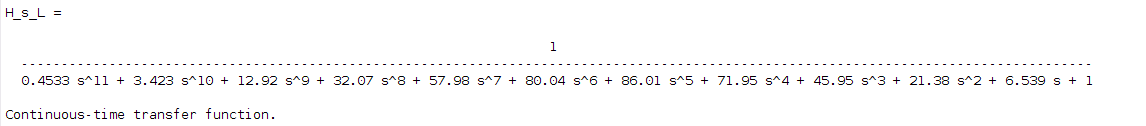
\includegraphics[width=1.2\textwidth, height=3cm]{images/Analog_but_lp_tf}
  \caption{Analog Low Pass Transfer Function }
  \label{fig:1}
\end{figure}
\begin{figure}[H]
  \centering
  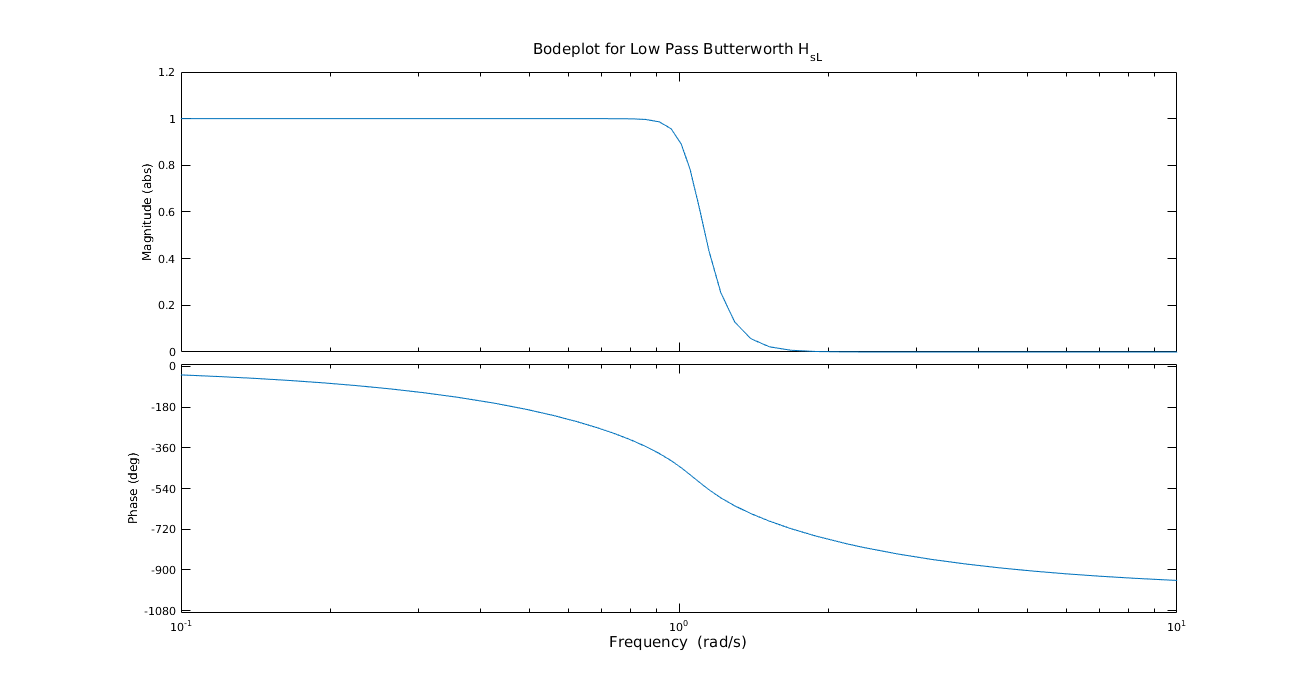
\includegraphics[scale=0.5]{images/Bodeplot_but_lp}
  \caption{Analog Low Pass Bode plot}
  \label{fig:2}
\end{figure}

\subsection{The Analog BandPass Transfer Function}
\begin{figure}[H]
  \centering
  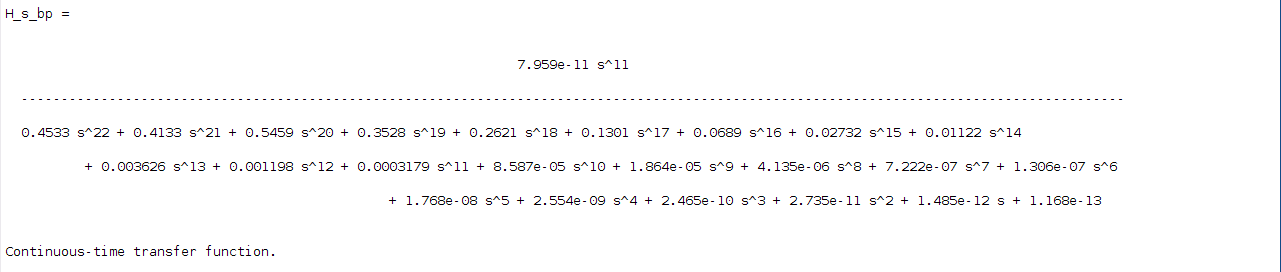
\includegraphics[width=1.2\textwidth,height=5cm]{images/Analog_but_bp_tf}
  \caption{Analog Band Pass Transfer Function}
  \label{fig:3}
\end{figure}
\begin{figure}[H]
  \centering
  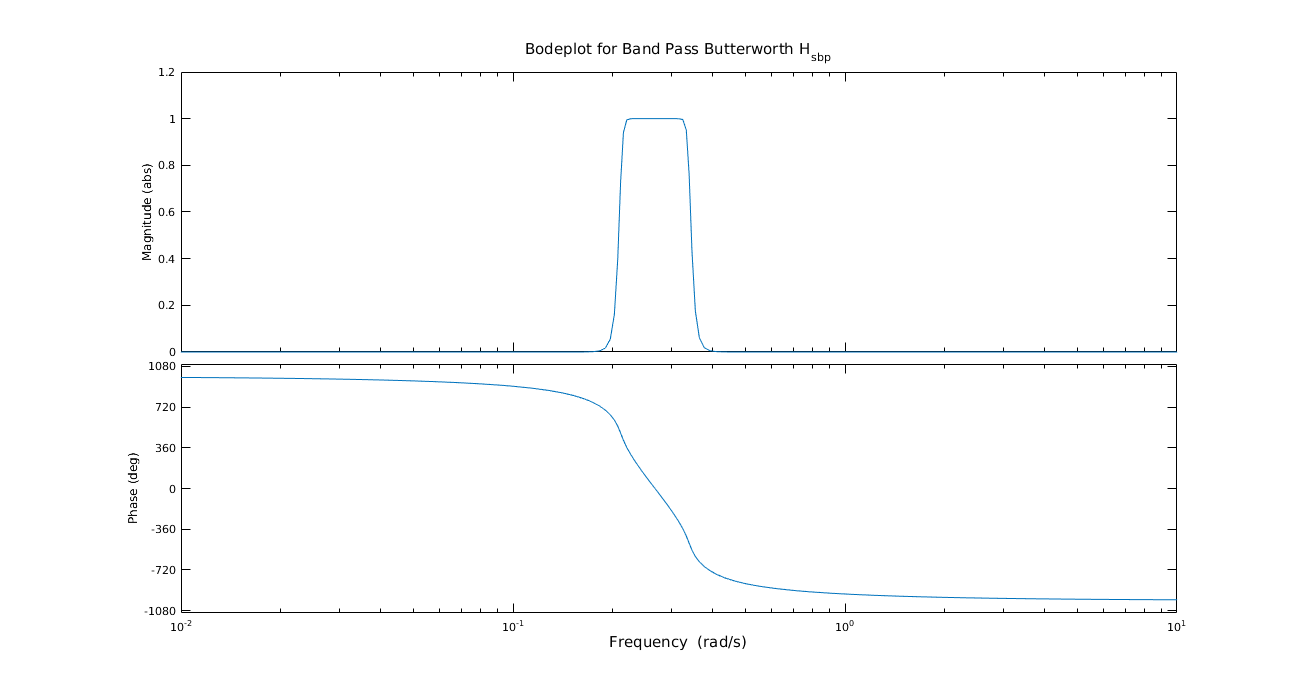
\includegraphics[scale=0.5]{images/Bodeplot_but_bp}
  \caption{Analog Band Pass Bode Plot}
  \label{fig:4}  
\end{figure}

\subsection{The Discrete Time Filter Transfer Function}
\begin{figure}[H]
  \centering
  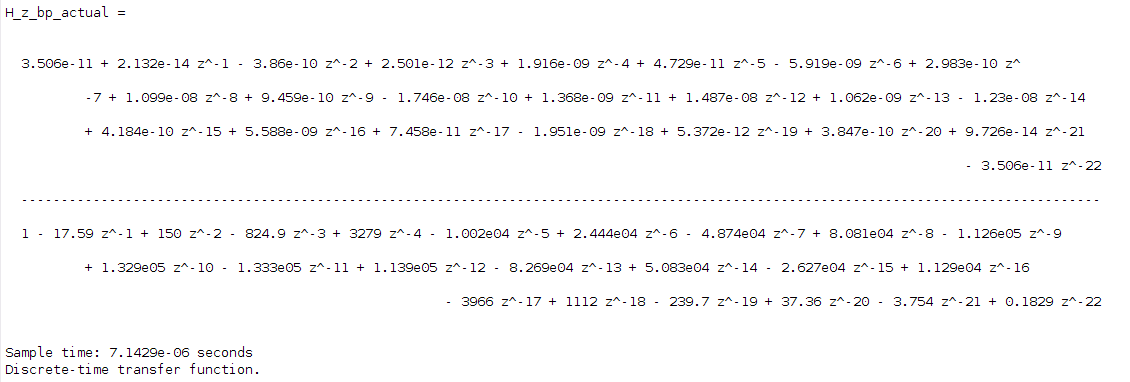
\includegraphics[width=1.2\textwidth,height=10cm]{images/Discrete_bp_tf}
  \caption{Discrete Time Band Pass Transfer Function}
  \label{fig:5}
\end{figure}
\begin{figure}[H]
  \centering
  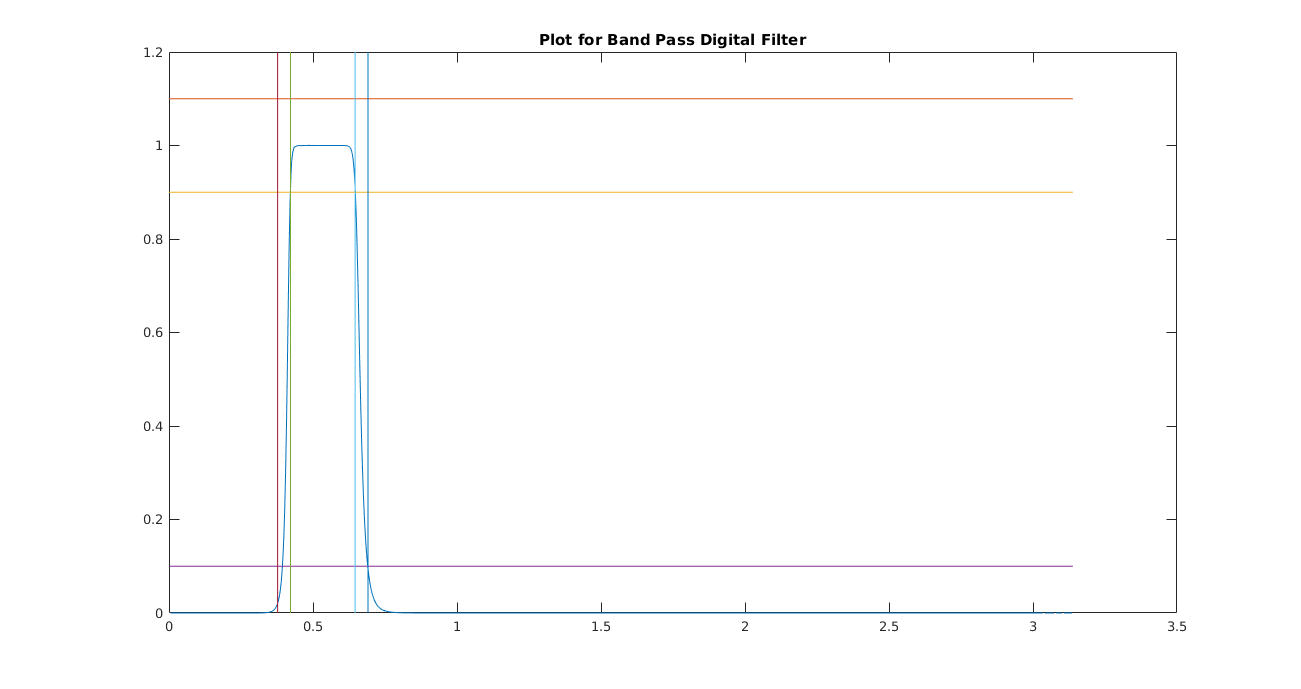
\includegraphics[scale=0.5]{images/Freqz_digital_bp}
  \caption{Frequency Magnitude Response of Discrete Time Band Pass Filter}
  \label{fig:6}
\end{figure}
% \newpage
% \vspace{-5cm}
\subsection{Direct Form 2 Realization of the Discrete Filter}
\begin{figure}[H]
  \centering
  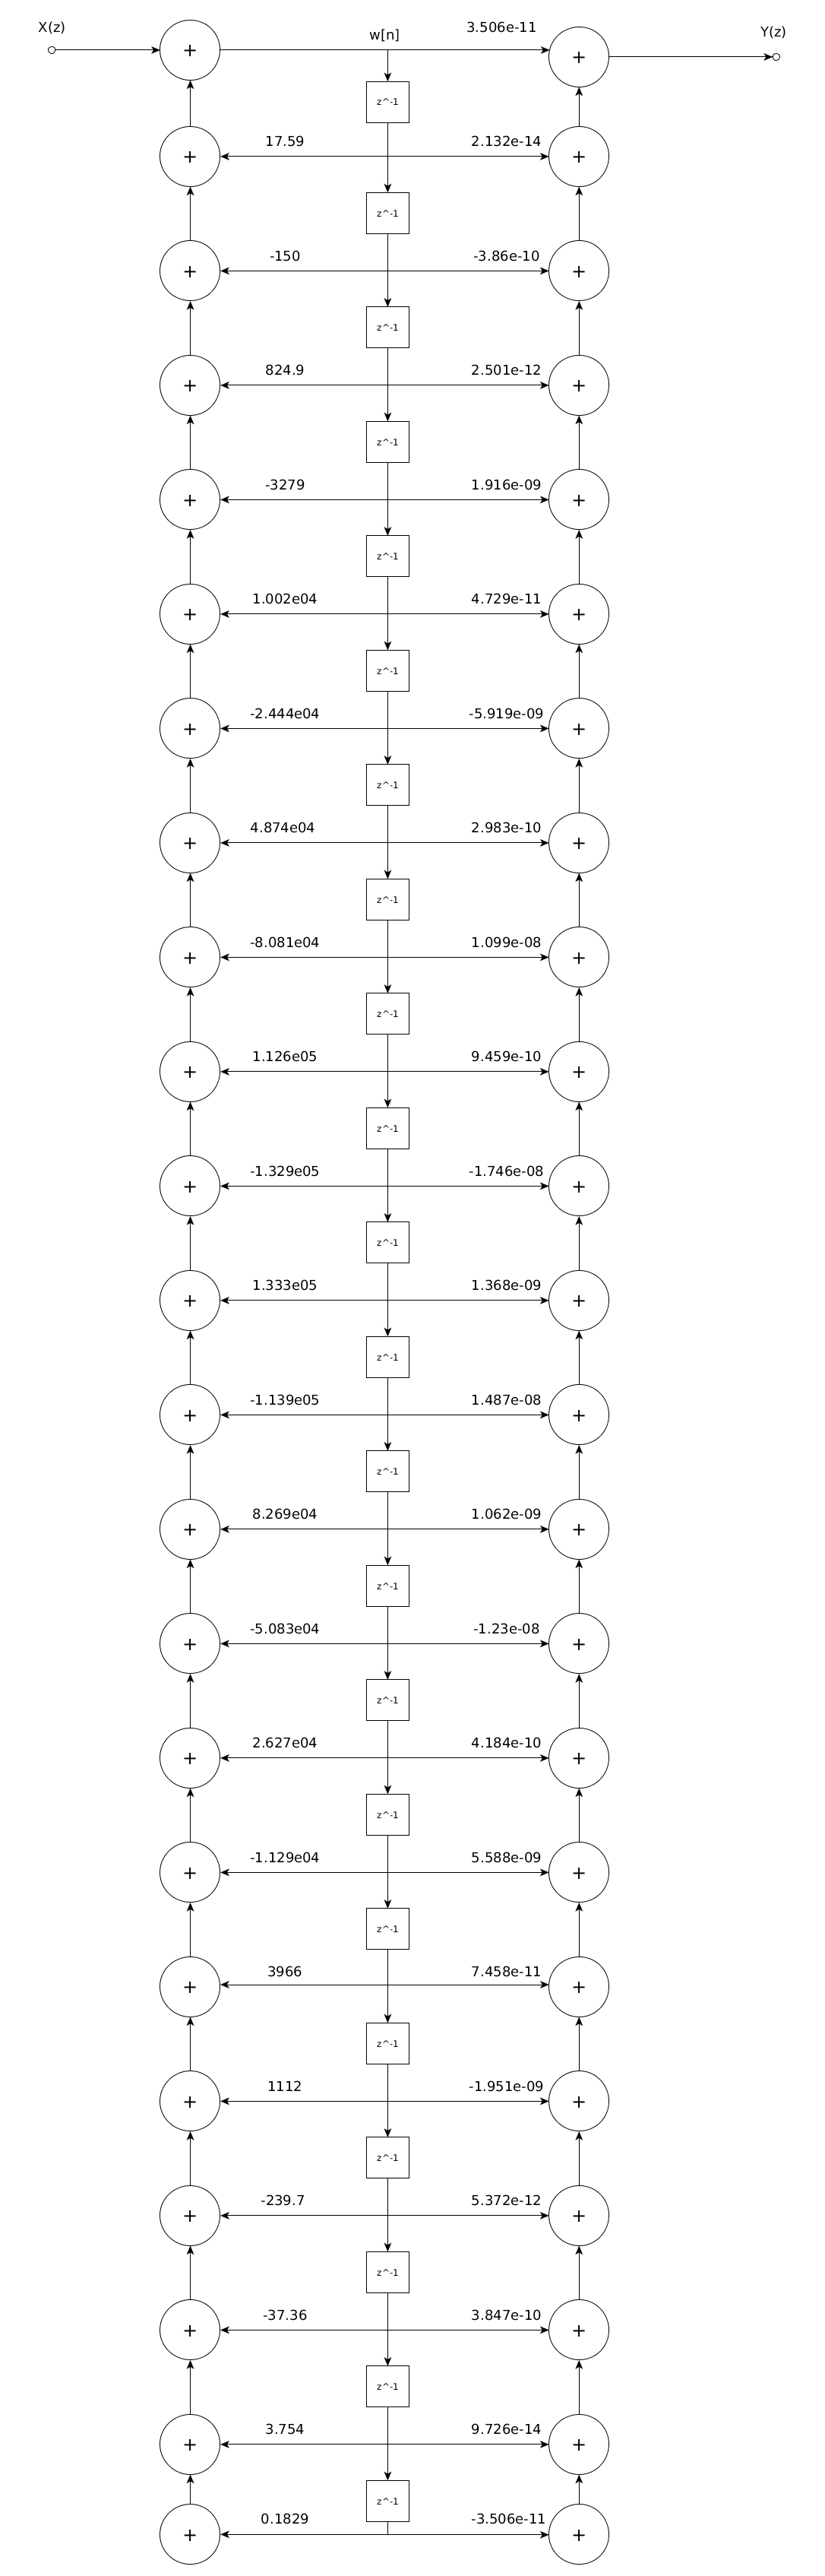
\includegraphics[scale=0.19]{images/direct_form2_bp}
  \caption{Direct Form 2 Signal Flow Graph for Band Pass IIR filter (Zoom In To see the Diagram)}
  \label{fig:7}
\end{figure}
\newpage
\subsection{FIR Filter Transfer Function to get the same specifications}
Given that $\delta = 0.1$, we get $$A = -20log_{10}(\delta) = -20log_{10}(0.1) = 20$$
For  $A < 21$ we get $\alpha = 0$ and hence $\beta = 0$.
Also we have $\Delta\omega = w_s - w_p$
We then compute $$N \ge \frac{A-8}{2*2.285*\Delta\omega} = 58.507$$
Therefore we choose $$N = 59$$.

But with $N = 59$ the resulting FIR doesn't meet all the specifications. Here is the plot for the same
\begin{figure}[H]
  \centering
  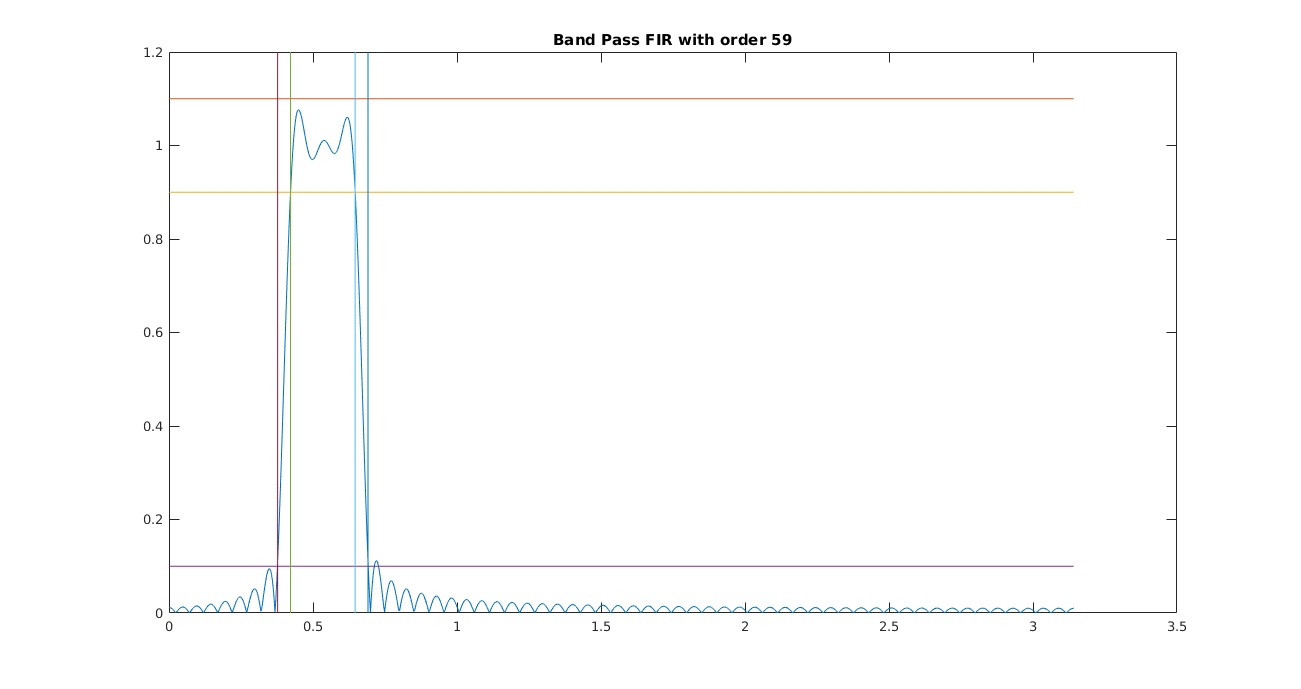
\includegraphics[scale=0.5]{images/Band_pass_fir_order_59}
  \caption{Order 59 FIR Band Pass}
  \label{fig:7}
\end{figure}

On increasing N to $N = 63$, we get an FIR that meets the specifications.
\begin{figure}[H]
  \centering
  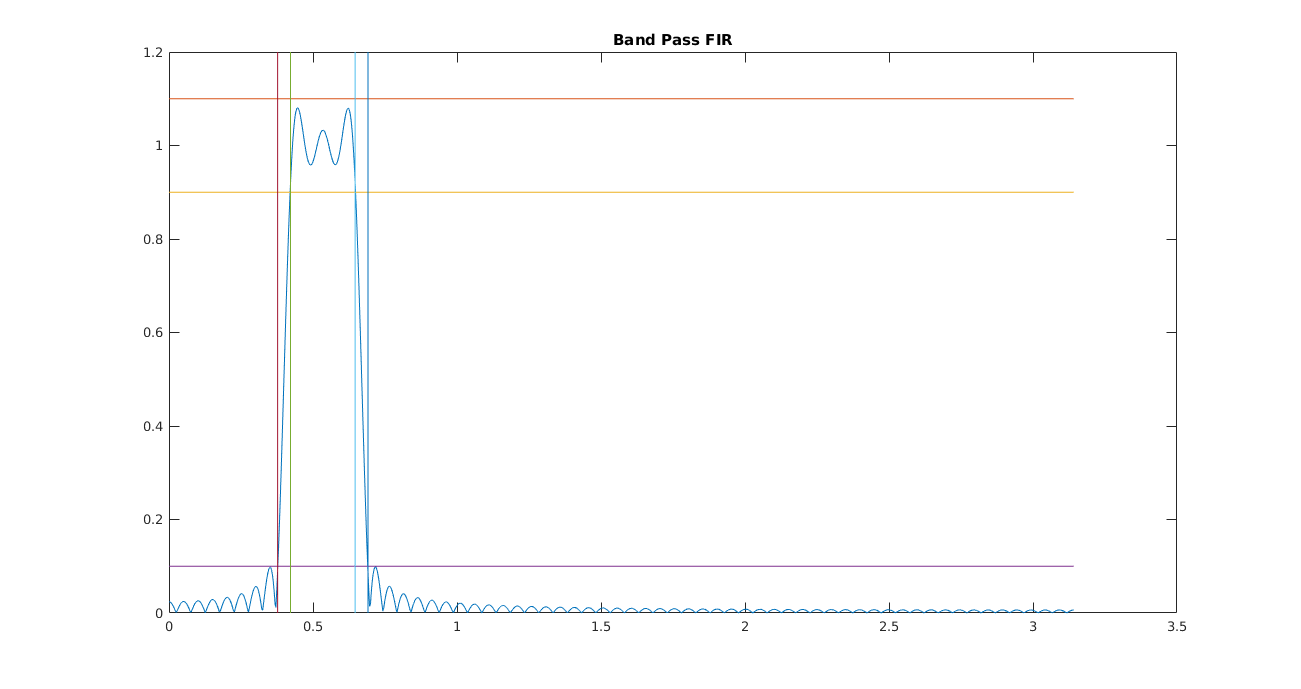
\includegraphics[scale=0.5]{images/Band_pass_fir_order_63}
  \caption{Order 63 FIR Band Pass}
  \label{fig:8}
\end{figure}

The complete Frequency Response is
\begin{figure}[H]
  \centering
  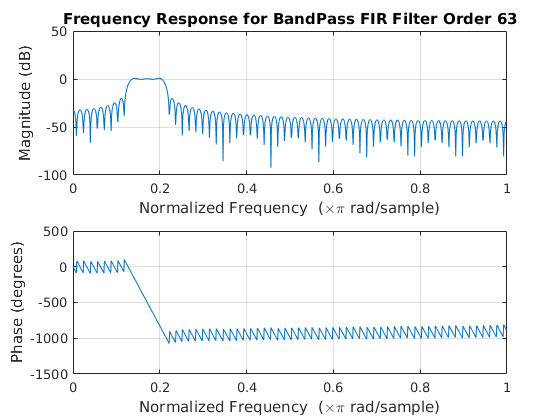
\includegraphics[scale=0.75]{images/FIR_bp_freqz}
  \caption{Frequency Response}
  \label{fig:9}
\end{figure}

$H_{fir\_bp} = 0.010699z^{-59} +0.0099216z^{-58} +0.0061769z^{-57} +0.00067888z^{-56} +-0.0047345z^{-55} +-0.0083073z^{-54} +-0.0090412z^{-53} +-0.0070586z^{-52} +-0.0035005z^{-51} +1.5549e-17z^{-50} +0.0020437z^{-49} +0.0020753z^{-48} +0.0006074z^{-47} +-0.0010474z^{-46} +-0.0014292z^{-45} +0.00031922z^{-44} +0.0039434z^{-43} +0.0080615z^{-42} +0.010683z^{-41} +0.010067z^{-40} +0.0055652z^{-39} +-0.0019308z^{-38} +-0.010166z^{-37} +-0.016293z^{-36} +-0.017965z^{-35} +-0.014297z^{-34} +-0.0062993z^{-33} +0.0034278z^{-32} +0.011658z^{-31} +0.015779z^{-30} +0.014805z^{-29} +0.009742z^{-28} +0.0031172z^{-27} +-0.0021396z^{-26} +-0.0040068z^{-25} +-0.0023031z^{-24} +0.0011925z^{-23} +0.003537z^{-22} +0.0020435z^{-21} +-0.0042678z^{-20} +-0.013846z^{-19} +-0.022858z^{-18} +-0.026534z^{-17} +-0.021167z^{-16} +-0.0059818z^{-15} +0.01592z^{-14} +0.038073z^{-13} +0.05258z^{-12} +0.052901z^{-11} +0.036481z^{-10} +0.0062323z^{-9} +-0.029837z^{-8} +-0.060854z^{-7} +-0.07654z^{-6} +-0.070733z^{-5} +-0.04374z^{-4} +-0.0026197z^{-3} +0.040796z^{-2} +0.073555z^{-1} +0.085714z^{0} +0.073555z^{1} +0.040796z^{2} +-0.0026197z^{3} +-0.04374z^{4} +-0.070733z^{5} +-0.07654z^{6} +-0.060854z^{7} +-0.029837z^{8} +0.0062323z^{9} +0.036481z^{10} +0.052901z^{11} +0.05258z^{12} +0.038073z^{13} +0.01592z^{14} +-0.0059818z^{15} +-0.021167z^{16} +-0.026534z^{17} +-0.022858z^{18} +-0.013846z^{19} +-0.0042678z^{20} +0.0020435z^{21} +0.003537z^{22} +0.0011925z^{23} +-0.0023031z^{24} +-0.0040068z^{25} +-0.0021396z^{26} +0.0031172z^{27} +0.009742z^{28} +0.014805z^{29} +0.015779z^{30} +0.011658z^{31} +0.0034278z^{32} +-0.0062993z^{33} +-0.014297z^{34} +-0.017965z^{35} +-0.016293z^{36} +-0.010166z^{37} +-0.0019308z^{38} +0.0055652z^{39} +0.010067z^{40} +0.010683z^{41} +0.0080615z^{42} +0.0039434z^{43} +0.00031922z^{44} +-0.0014292z^{45} +-0.0010474z^{46} +0.0006074z^{47} +0.0020753z^{48} +0.0020437z^{49} +1.5549e-17z^{50} +-0.0035005z^{51} +-0.0070586z^{52} +-0.0090412z^{53} +-0.0083073z^{54} +-0.0047345z^{55} +0.00067888z^{56} +0.0061769z^{57} +0.0099216z^{58} +0.010699z^{59}$



\section{Second Filter Specifications}
% \begin{enumerate}
\subsection{Un-normalized Discrete Time Filter Specifications}
\begin{itemize}
\item Sampling Frequency ($f_s$) = 90kHz
\item $B_L = 7.7 kHz$
\item $B_H = 10.7 kHz$
\item Equiripple Passband (Chebyshev)
\end{itemize}
\subsection{Normalized Digital Filter Specifications}
\begin{itemize}
\item $\omega_{p1} = \frac{6.7}{90}2\pi = 0.4677$
\item $\omega_{p2} = \frac{11.7}{90}2\pi = 0.8168$
\item $\omega_{s1} = \frac{7.7}{90}2\pi = 0.5376$
\item $\omega_{s2} = \frac{10.7}{90}2\pi = 0.7470$
\end{itemize}
\subsection{Analog Filter Specifications}
\begin{itemize}
\item $\Omega_{p1} = tan(\frac{\omega_{p1}}{2}) = 0.2382$ 
\item $\Omega_{p2} = tan(\frac{\omega_{p2}}{2}) = 0.4327$
\item $\Omega_{s1} = tan(\frac{\omega_{s1}}{2}) = 0.2754$
\item $\Omega_{s2} = tan(\frac{\omega_{s2}}{2}) = 0.3919$
\end{itemize}
\subsection{Frequency transformation to be employed}
\begin{equation}
  \label{eq:3}
  s_L = \frac{Bs}{s^2 + \Omega_0^2}
\end{equation}
with $B = \Omega_{p2} - \Omega_{p1} = 0.1945$ and $\Omega_0 = \sqrt{\Omega_{p1}\Omega_{p2}} = 0.3211$
\\  This translates to
\begin{equation}
  \label{eq:4}
  \Omega_{L} = \frac{B\Omega}{\Omega^2 - \Omega_0^2}
\end{equation}
\subsection{Frequency transformed lowpass analog filter specifications}
From \ref{eq:4}
\begin{itemize}
\item $\Omega_{Lp} = 1$
\item $\Omega_{Ls} = min(\Omega_{Ls1},\Omega_{Ls2}) = 1.5097$
\end{itemize}

\subsection{The analog Low pass Transfer Function}
\begin{figure}[H]
  \centering
  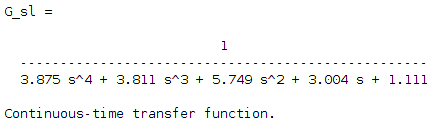
\includegraphics[height=3cm]{images/Analog_cheb_lp_tf}
  \caption{Analog Low Pass Transfer Function For Band Stop}
  \label{fig:9}
\end{figure}
\begin{figure}[H]
  \centering
  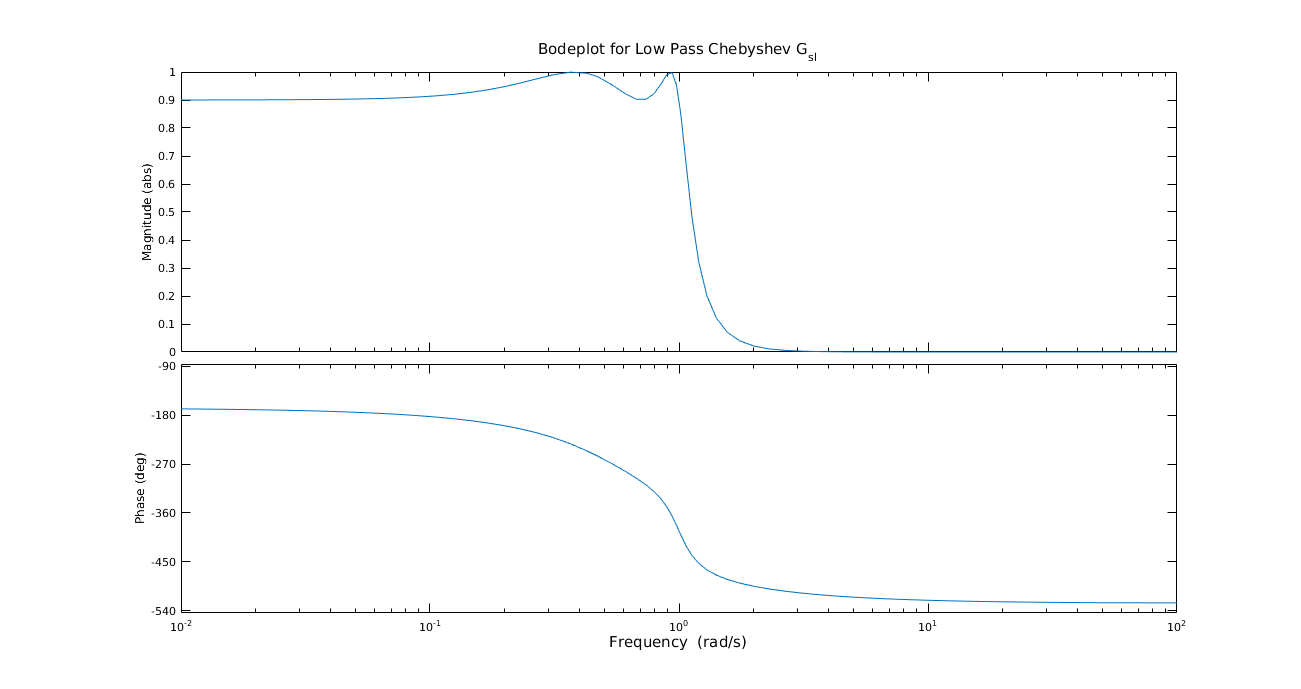
\includegraphics[scale=0.5]{images/Bodeplot_cheb_lp}
  \caption{Analog Low Pass Bode plot For Band Stop}
  \label{fig:10}
\end{figure}

\subsection{The Analog BandStop Transfer Function}
\begin{figure}[H]
  \centering
  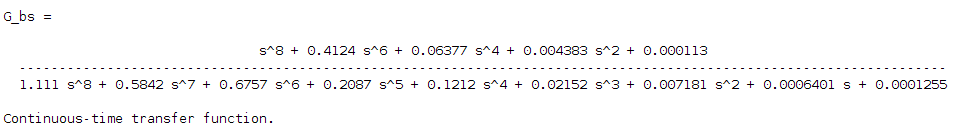
\includegraphics[width=1.2\textwidth,height=3cm]{images/Analog_cheb_bs_tf}
  \caption{Analog Band Stop Transfer Function}
  \label{fig:11}
\end{figure}
\begin{figure}[H]
  \centering
  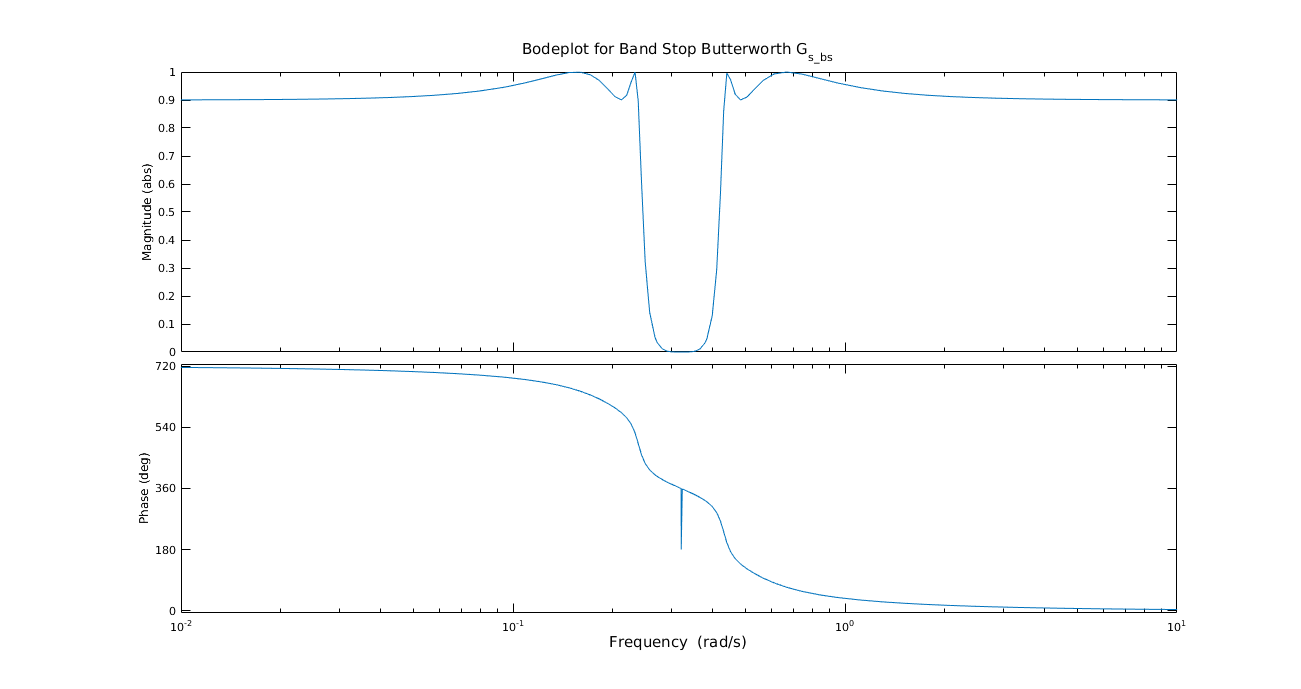
\includegraphics[scale=0.5]{images/Bodeplot_cheb_bs}
  \caption{Analog Band Stop Bode Plot}
  \label{fig:12}  
\end{figure}

\subsection{The Discrete Time Filter Transfer Function}
\begin{figure}[H]
  \centering
  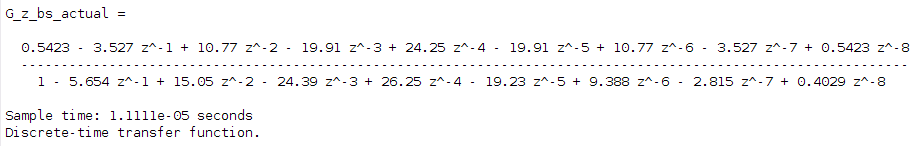
\includegraphics[width=1.2\textwidth,height=3cm]{images/Discrete_bs_tf}
  \caption{Discrete Time Band Stop Transfer Function}
  \label{fig:13}
\end{figure}
\begin{figure}[H]
  \centering
  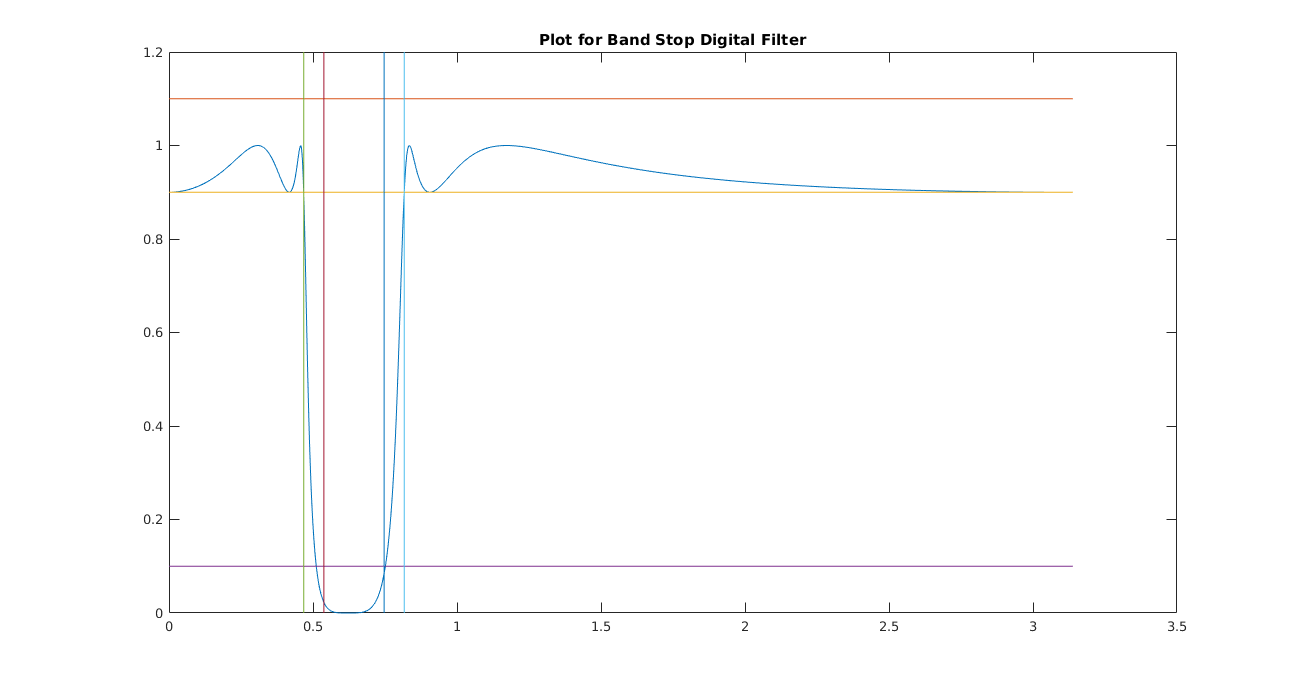
\includegraphics[scale=0.5]{images/Freqz_digital_bs}
  \caption{Frequency Magnitude Response of Discrete Time Band Stop Filter}
  \label{fig:14}
\end{figure}
% \newpage
% \vspace{-5cm}
\subsection{Direct Form 2 Realization of the Discrete Filter}
\begin{figure}[H]
  \centering
  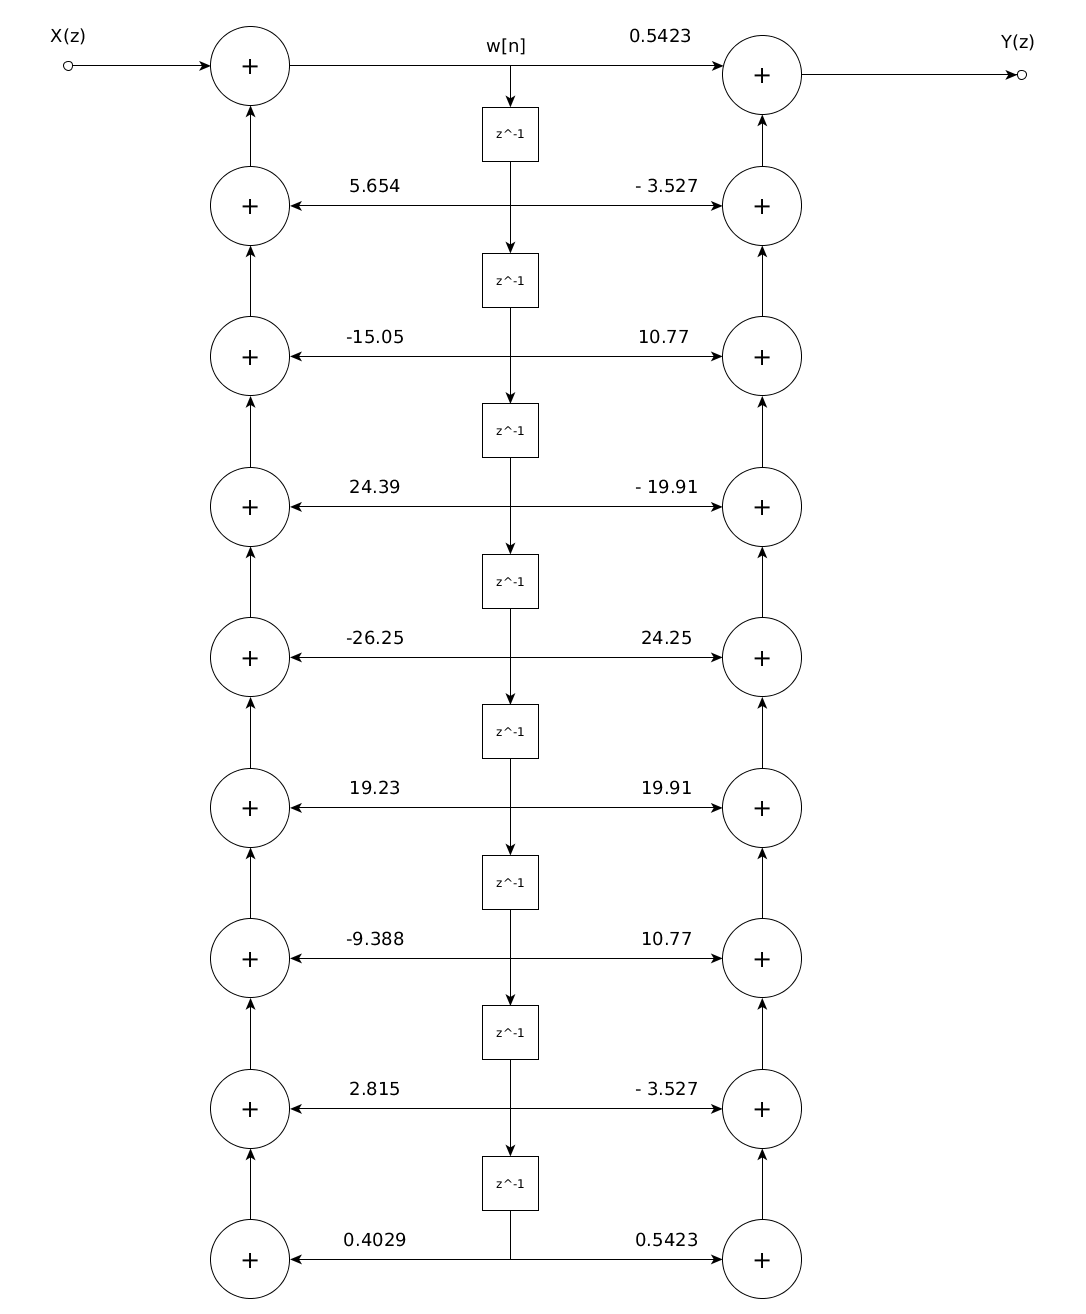
\includegraphics[scale=0.3]{images/direct_form2_bs}
  \caption{Direct Form 2 Signal Flow Graph for Band Stop IIR filter (Zoom In To see the Diagram)}
  \label{fig:15}
\end{figure}
\newpage
\subsection{FIR Filter Transfer Function to get the same specifications}
Given that $\delta = 0.1$, we get $$A = -20log_{10}(\delta) = -20log_{10}(0.1) = 20$$
For  $A < 21$ we get $\alpha = 0$ and hence $\beta = 0$.
Also we have $\Delta\omega = w_s - w_p$
We then compute $$N \ge \frac{A-8}{2*2.285*\Delta\omega} = 37.6121$$
Therefore we choose $$N = 38$$.

But with $N = 38$ the resulting FIR doesn't meet all the specifications. Here is the plot for the same
\begin{figure}[H]
  \centering
  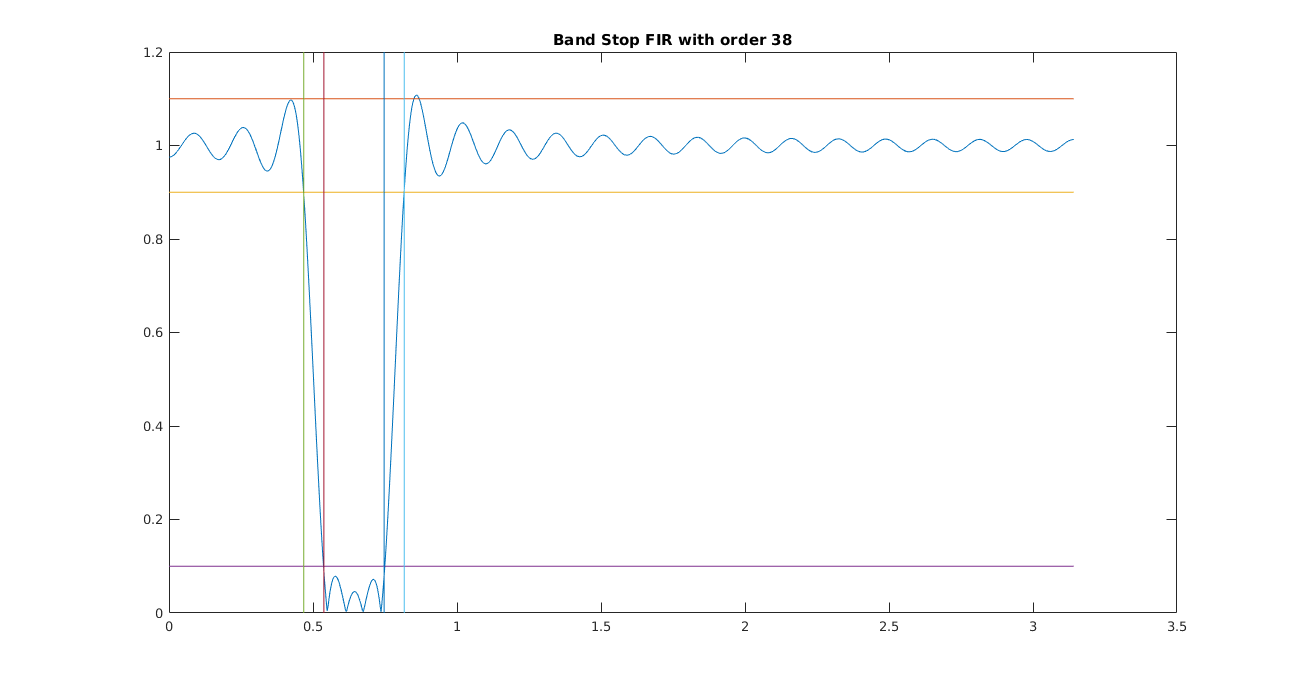
\includegraphics[scale=0.5]{images/Band_stop_fir_order_38}
  \caption{Order 38 FIR Band Stop}
  \label{fig:7}
\end{figure}

On increasing N to $N = 39$, we get an FIR that meets the specifications.
\begin{figure}[H]
  \centering
  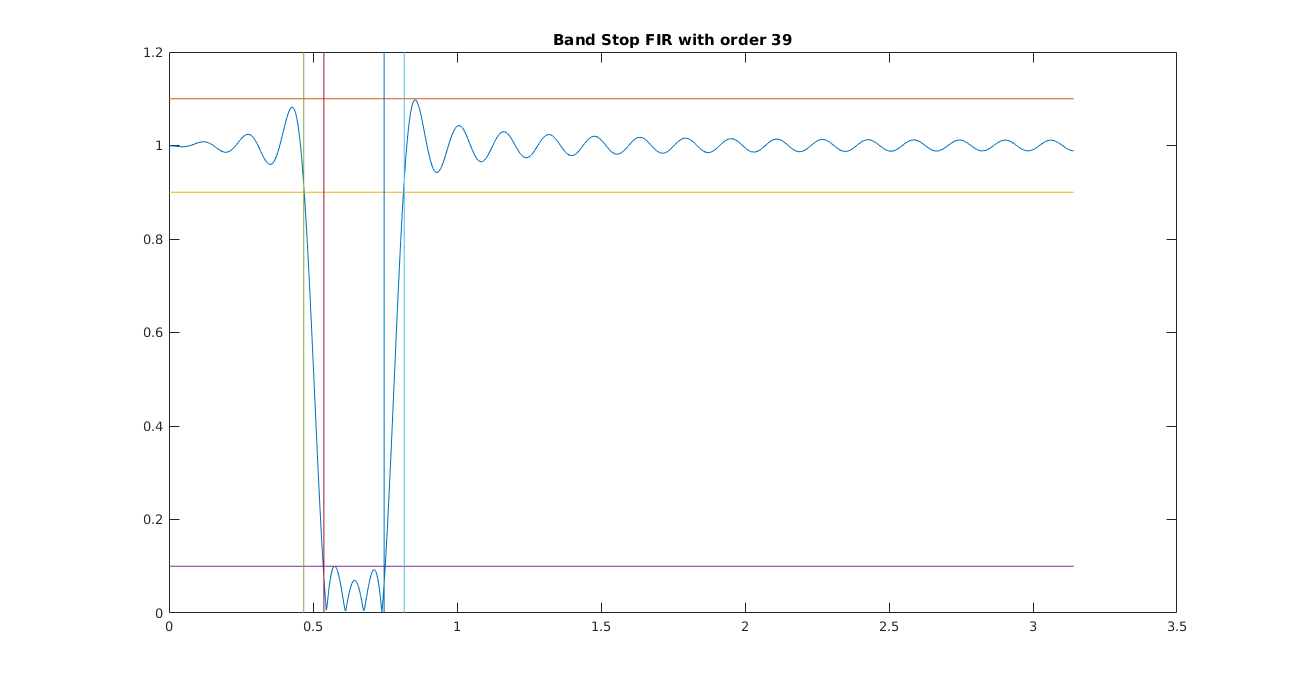
\includegraphics[scale=0.5]{images/Band_stop_fir_order_39}
  \caption{Order 39 FIR Band Stop}
  \label{fig:8}
\end{figure}


The complete Frequency Response is
\begin{figure}[H]
  \centering
  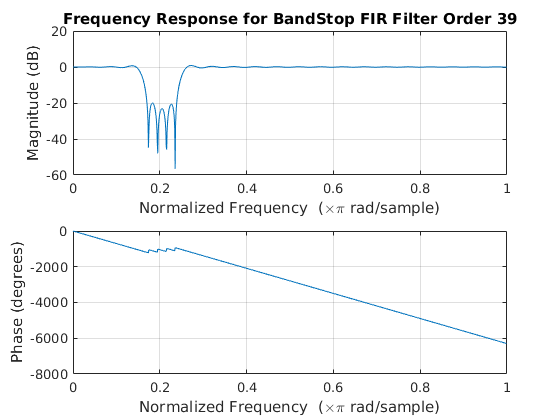
\includegraphics[scale=0.75]{images/FIR_bs_freqz}
  \caption{Frequency Response}
  \label{fig:9}
\end{figure}


$H_{fir\_bs} = 0.012088z^{-39} +0.010386z^{-38} +0.0031096z^{-37} +-0.0071609z^{-36} +-0.015816z^{-35} +-0.018492z^{-34} +-0.013424z^{-33} +-0.002553z^{-32} +0.0092892z^{-31} +0.016789z^{-30} +0.016869z^{-29} +0.010236z^{-28} +0.00087022z^{-27} +-0.0062943z^{-26} +-0.0081842z^{-25} +-0.0052796z^{-24} +-0.0011458z^{-23} +-1.4092e-05z^{-22} +-0.0038107z^{-21} +-0.010465z^{-20} +-0.014705z^{-19} +-0.011139z^{-18} +0.0019957z^{-17} +0.020653z^{-16} +0.035952z^{-15} +0.038273z^{-14} +0.0226z^{-13} +-0.0077075z^{-12} +-0.041041z^{-11} +-0.062085z^{-10} +-0.058952z^{-9} +-0.029547z^{-8} +0.01619z^{-7} +0.059689z^{-6} +0.081643z^{-5} +0.070893z^{-4} +0.030086z^{-3} +-0.024772z^{-2} +-0.070945z^{-1} +0.91111z^{0} +-0.070945z^{1} +-0.024772z^{2} +0.030086z^{3} +0.070893z^{4} +0.081643z^{5} +0.059689z^{6} +0.01619z^{7} +-0.029547z^{8} +-0.058952z^{9} +-0.062085z^{10} +-0.041041z^{11} +-0.0077075z^{12} +0.0226z^{13} +0.038273z^{14} +0.035952z^{15} +0.020653z^{16} +0.0019957z^{17} +-0.011139z^{18} +-0.014705z^{19} +-0.010465z^{20} +-0.0038107z^{21} +-1.4092e-05z^{22} +-0.0011458z^{23} +-0.0052796z^{24} +-0.0081842z^{25} +-0.0062943z^{26} +0.00087022z^{27} +0.010236z^{28} +0.016869z^{29} +0.016789z^{30} +0.0092892z^{31} +-0.002553z^{32} +-0.013424z^{33} +-0.018492z^{34} +-0.015816z^{35} +-0.0071609z^{36} +0.0031096z^{37} +0.010386z^{38} +0.012088z^{39}$


\end{document}


